% CVPR 2027 official review template version adapted for TLIR.
\documentclass[10pt,twocolumn,letterpaper]{article}
\usepackage[review]{cvpr}
%% This file contains a number of tweaks that are typically applied to the main document.
%% They are not enabled by default, but can be enabled by uncommenting the relevant lines.

%%
%% Inline annotations; for predefined colors, refer to "dvipsnames" in the xcolor package:
%% https://tinyurl.com/overleaf-colors
%%
\newcommand{\red}[1]{{\color{red}#1}}
\newcommand{\todo}[1]{{\color{red}#1}}
\newcommand{\TODO}[1]{\textbf{\color{red}[TODO: #1]}}
%%
%% disable for camera ready / submission by uncommenting these lines  
%%
% \renewcommand{\TODO}[1]{}
% \renewcommand{\todo}[1]{#1}

%%
%% work harder in optimizing text layout. Typically shrinks text by 1/6 of page, enable
%% it at the very end of the writing process, when you are just above the page limit
%%
% \usepackage{microtype}

%%
%% fine-tune paragraph spacing
%%
% \renewcommand{\paragraph}[1]{\vspace{.5em}\noindent\textbf{#1.}}

%%
%% globally adjusts space between figure and caption
%%
% \setlength{\abovecaptionskip}{.5em}


%%
%% Allows "the use of \paper to refer to the project name"
%% with automatic management of space at the end of the word
%%
% \usepackage{xspace}
% \newcommand{\paper}{ProjectName\xspace}

%%
%% Commonly used math definitions
%%
% \DeclareMathOperator*{\argmin}{arg\,min}
% \DeclareMathOperator*{\argmax}{arg\,max}

%%
%% Tigthen underline
%%
% \usepackage{soul}
% \setuldepth{foobar}
\usepackage{times}
\usepackage[utf8]{inputenc}
\usepackage{url}
\usepackage{array}
\usepackage{amsmath,amssymb}
\usepackage{booktabs}
\definecolor{cvprblue}{rgb}{0.21,0.49,0.74}
\usepackage[pagebackref,breaklinks,colorlinks,allcolors=cvprblue]{hyperref}
\urlstyle{same}
\def\confName{CVPR}
\def\confYear{2027}
\hypersetup{pdfauthor={},pdftitle={Unified Training--Learning--Inference--Reinforcement Dynamics Across Neural Systems}}
\newcommand{\dd}{\Delta\theta_t}
\newcommand{\id}{\mathrm{id}}
\newcommand{\PASS}{\textsc{Pass}}
\title{Unified Training--Learning--Inference--Reinforcement Dynamics Across Neural Systems}
\author{Anonymous CVPR Submission}
\begin{document}
\maketitle
\begin{abstract}
We study unified Training--Learning--Inference--Reinforcement (TLIR) dynamics across neural systems. Training evolves a parameter--optimizer state: the same realized update can produce different finite-amplitude functional responses in different receiving states. Learning persistently reorganizes distributed functional support, and a target's capability changes when its readout boundary is crossed. Inference recruits and combines learned support at a frozen persistent state; reinforcement couples environmental consequences to subsequent training actions. We establish the connected Training--Learning--Inference (TLI) relations in nanoGPT and test them in ResNet-18, diffusion U-Net, routed Vision-MoE, a graph neural network, and a hard-spiking recurrent network. The experiments include realized-update exchanges, finite-amplitude response paths, component-coalition interventions, target-boundary measurements, and exact trained-version inference rollback. A theory-derived target-boundary predictor classifies immediate outcomes of formed updates across architectures. In a seventh, shared GRU policy, RL-E05/E06 examine how correct-feedback concentration changes functional support, weakens other mastered skills, and enables recovery when feedback is redistributed. The combined results provide an experimentally traceable account of training actions, learning, inference, and reinforcement.
\end{abstract}
\section{Introduction}
Training, generalization, capability formation, and inference are central problems in neural-network research. Different fields have developed influential theories to study them.

In \emph{optimization theory}, the Neural Tangent Kernel (NTK) describes parameter-induced output changes through the network Jacobian and the corresponding kernel in specified training regimes \cite{jacot2018}. Edge of Stability studies training behavior in relation to the largest Hessian eigenvalue, learning rate, and loss trajectory \cite{cohen2021}. Sharpness-Aware Minimization (SAM) constructs training updates using loss changes in a parameter neighborhood to improve generalization \cite{foret2021}. Here, the \emph{current state} is represented by parameters and their local derivatives or curvature; \emph{realized updates} are produced by the optimizer; and \emph{responses} appear as changes in model outputs or loss.

In \emph{representation learning and generalization}, Spectral Bias examines frequency-dependent learning rates of functions or kernel modes \cite{rahaman2019}. Implicit Bias studies why an optimizer selects particular solutions, such as maximum-margin directions on separable data \cite{soudry2018}. Neural Collapse measures class-feature means, within-class variability, and classifier geometry, revealing continuing representational change after training accuracy saturates \cite{papyan2020}. Information Bottleneck theory studies mutual information among inputs, hidden representations, and targets, including the retention and compression of task-relevant information \cite{tishby2015}. Their \emph{internal organizations} take the form of spectral modes, optimizer-selected solutions, feature geometry, or information structure; their \emph{functional changes} appear in learning rates, evolving solutions, and predictive performance.

In \emph{capability formation}, Grokking captures the long delay between fitting training examples and achieving strong test generalization \cite{power2022}. Subsequent circuit studies track the formation and reorganization of internal computations during this delay \cite{nanda2023}. Double Descent studies how test error can rise near interpolation and fall again as model size, training time, or data conditions change \cite{belkin2019,nakkiran2020}. These studies measure the \emph{current state} through training phase or interpolation regime, \emph{internal change} through circuit and solution evolution, and \emph{observable capability} through accuracy and generalization error.

In \emph{continual learning}, catastrophic forgetting occurs when training on a new task reduces performance on earlier tasks. Elastic Weight Consolidation (EWC) estimates parameter importance using Fisher information from earlier tasks and penalizes changes to important parameters \cite{kirkpatrick2017}. Gradient Episodic Memory (GEM) constrains new-task gradients using their inner products with previous-task gradients \cite{lopezpaz2017}. Orthogonal Gradient Descent (OGD) projects new gradients into directions that approximately preserve earlier-task outputs \cite{farajtabar2020}. In these methods, the \emph{existing state} includes previously learned parameters and function-sensitive directions; \emph{updates} are constrained new-task actions; \emph{interactions} occur through overlapping gradient or functional subspaces; and \emph{capability changes} are measured as retention, forgetting, or transfer.

In \emph{inference research}, Attention uses queries, keys, and values to compute input-dependent information weights \cite{vaswani2017}. In-context learning studies how examples and task information provided in the context affect predictions while model parameters remain fixed \cite{brown2020}. Chain-of-Thought prompting studies how intermediate reasoning steps affect performance on complex tasks \cite{wei2022}. The \emph{current state} is the trained model; \emph{input conditions} include the query, context, and intermediate computations; \emph{internal computation} varies with attention and activations; and \emph{functional performance} is observed in the resulting predictions.

In \emph{reinforcement and feedback-driven training}, reinforcement learning from human feedback (RLHF) uses preference and reward signals to adjust model behavior \cite{ouyang2022}. Self-training creates further training data from a model's predictions \cite{xie2020}. Recursive model-collapse studies examine the loss of low-probability modes when successive models are trained on data generated by their predecessors \cite{shumailov2024}. Here, \emph{feedback} is supplied through rewards, preferences, or generated-data distributions; \emph{training actions} are the resulting updates; and subsequent \emph{functional change} is observed through behavior, accuracy, and generated distributions.

These studies use different mathematical objects---kernels, Hessians, gradients, class features, mutual information, task scores, attention weights, and reward signals---yet six recurring categories can be identified: \emph{current state, realized update, functional response, internal organization, observable capability, and feedback}. \emph{The core TLI relations were established experimentally before this cross-field comparison; identifying these recurring variables here is a way to help readers understand the theory, not the process by which it was discovered.}


\begin{figure*}[t]
  \centering
  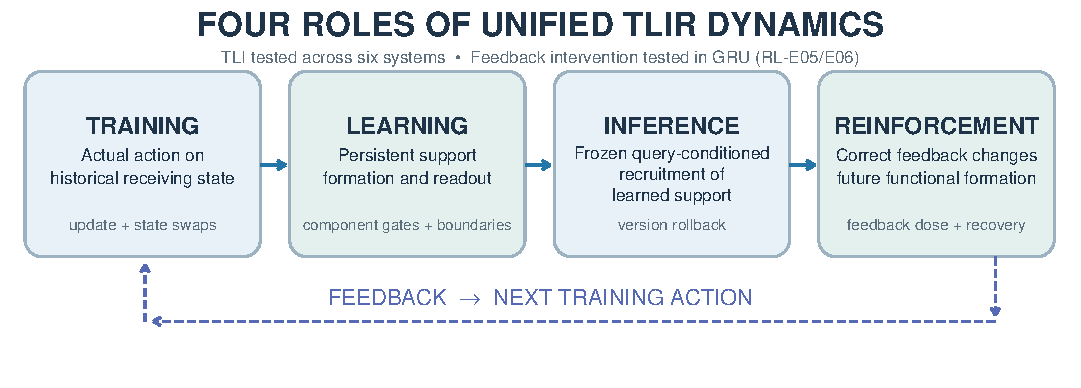
\includegraphics[width=.98\textwidth]{figures/figure1_functional_chain.pdf}
  \caption{Four peer roles of TLIR. The TLI core is tested in six neural systems; RL-E05/E06 test reinforcement through controlled feedback redistribution in a shared GRU policy.}
  \label{fig:chain}
\end{figure*}


\section{Experimental Systems and Methods}
\subsection{Neural systems and indexed experiments}
The TLI core was established in nanoGPT through TL-E01--E08 and INF-E01, with TL-P01 testing a predictive consequence. Five additional systems retest its connected roles. RL-E05/E06 examine how correct feedback reallocates already learned functional support and changes retained capabilities in a seventh system, a shared GRU policy. Table~\ref{tab:systems} lists the executed systems and registered component groups.

\begin{table}[t]
\centering\small\setlength{\tabcolsep}{3pt}\renewcommand{\arraystretch}{1.07}
\begin{tabular}{@{}>{\raggedright\arraybackslash}p{.40\columnwidth}>{\raggedright\arraybackslash}p{.54\columnwidth}@{}}
\toprule
System (optimizer) & Task / registered components\\
\midrule
nanoGPT (Adam) & Cyclic next-token; 4 attention/MLP branches\\
ResNet-18 (SGD momentum) & CIFAR-100 classification; 4 residual stages\\
Diffusion U-Net\newline(AdamW) & CIFAR-10 denoising; 4 U-Net paths\\
Vision-MoE (AdamW) & CIFAR-100 classification; 4 routed experts\\
GNN (RMSprop) & Graph reachability; 4 message-passing blocks\\
Spiking SNN (Adagrad) & 8$\times$8 digits; 4 spiking blocks\\
GRU (RL-E05/E06; AdamW) & Four-skill feedback; 4 shared hidden groups\\
\bottomrule
\end{tabular}
\caption{Seven neural systems: six TLI chains and a GRU feedback study.}
\label{tab:systems}
\end{table}

\subsection{Training: realized actions and receiving states}
At a registered update, the actual model--optimizer state is $Z_t=(\theta_t,\omega_t)$, with realized parameter action $\Delta\theta_t=\theta_{t+1}-\theta_t$. The experiment records the pre-state, minibatch, gradient, optimizer memory, and native post-state. TL-E01/E02 examine capability trajectories and optimizer-pause/clipping controls. TL-E03 transplants an \emph{identical formed update} between historical receiving states and compares responses relative to each unchanged-state branch:
\begin{equation}
 R_q(\theta_A,\Delta\theta_B)\quad\text{vs.}\quad R_q(\theta_B,\Delta\theta_B),
 \label{eq:receiver}
\end{equation}
where $R_q(\theta,\Delta)=m_q(\theta+\Delta)-m_q(\theta)$ for target $q$. A separate optimizer-memory fork fixes the current parameters and gradient while substituting historical memory:
\begin{equation}
 \Delta^{(a,b)}=\operatorname{OptStep}(\theta_t,g_t,\omega_{a,b}).
 \label{eq:optmem}
\end{equation}
TL-E04 evaluates the \emph{realized} update at finite amplitudes,
\begin{equation}
 r_{t,q}(\alpha)=m_q(\theta_t+\alpha\Delta\theta_t)-m_q(\theta_t),
 \label{eq:response}
\end{equation}
with common cross-system grid $\alpha\in\{0,.125,.25,.5,.75,1\}$. The paths reveal linear, saturation, acceleration, turnback, and sign-reversal regimes. TL-E05 identifies three main pre-response conditioning families: current target-boundary state (F1), target-specific update geometry (F3), and parameter--optimizer receiving state (F5).

\subsection{Learning: support formation and readout}
TL-E06 applies reversible zero gates to identified components. For active coalition $C\subseteq\mathcal C$, let $v_{t,q}(C)=m_q(f_{\theta_t}^{(C)}(x_q))$. Single/pair interventions measure necessity, backup, substitution, interaction, and failure slack; cross-system implementations also evaluate the 16 coalitions of four components and their exact Shapley effects:
\begin{equation}
 \phi_{j,q}=\!\!\sum_{C\subseteq\mathcal C\setminus\{j\}}
 \frac{|C|!(3-|C|)!}{4!}\left[v_q(C\cup\{j\})-v_q(C)\right].
 \label{eq:shapley}
\end{equation}
TL-E07 compares the intervention-derived support allocation before and after the \emph{same} update,
\begin{equation}
 \Delta P_{t,q}=P_q(\theta_t+\Delta\theta_t)-P_q(\theta_t),
 \label{eq:realloc}
\end{equation}
including support hand-offs and component interactions. TL-E08 aligns identities and target readout boundaries. Classifiers use $m_q=\ell_y-\max_{c\ne y}\ell_c$; diffusion uses a native residual-competition boundary $m_q=\min_k(E_k-E_{\mathrm{true}})$. The pre/post signs give four outcomes: $(1,1)$, $(1,0)$, $(0,0)$, and $(0,1)$ for maintenance, loss, non-acquisition, and recovery/acquisition.

\subsection{Inference: frozen recruitment and rollback}
INF-E01 tests 13 nanoGPT histories and 52 identified checkpoints; INF-G01/G02 and the GNN/SNN studies extend these measurements. At a fixed learned state $L^*$, inference recruits query-conditioned support and combines it in the current occurrence:
\begin{equation}
 S_{q,c}^{\mathrm{active}}=\Pi_{q,c}(L^*),\qquad
 y_{q,c}=H_{q,c}(S_{q,c}^{\mathrm{active}}).
 \label{eq:inference}
\end{equation}
Frozen component gates measure non-additivity at the \emph{complete output} level:
\begin{equation}
 I_{ij,q}=f_{\mathrm{full}}-f_{-i}-f_{-j}+f_{-i,-j}.
 \label{eq:interaction}
\end{equation}
Each trained component is separately replaced by its exact pre-learning version, while other trained parameters remain fixed; its output effect is
\begin{equation}
 D_{j,q}=f(q;\theta^*)-f(q;\theta^{(j\leftarrow\mathrm{pre})}).
 \label{eq:rollback}
\end{equation}
The original trained version is then restored, with the output and persistent model/optimizer state checked for exact recovery.

\subsection{Reinforcement: correct-feedback redistribution}
Reinforcement is a peer TLIR role, not an add-on to TLI. RL-E05 and RL-E06 begin with a shared attention-free GRU policy in which \emph{four capabilities have reached mastery}. All branches receive matched initial parameter--AdamW states. A complete two-decision chain receives $r=1$ only when correct and $r=0$ otherwise. The interventions manipulate \emph{where correct feedback is concentrated}, not the reward rule.

RL-E05 compares selective feedback for one mastered capability, balanced feedback for all four, and frozen exposure without parameter updates. All 16 coalitions of four GRU component groups measure Shapley support and task margins; 15 nonempty component-version rollback subsets test the observed capability trade-off.

RL-E06 holds 60 episodes per update and the 3,200-update budget constant while varying feedback allocation (Table~\ref{tab:dose}). At exclusive-feedback update 800, two exact-state recovery forks receive 2,400 further updates: rebalanced $[15,15,15,15]$ or other-skills-only $[0,20,20,20]$. Feedback dose, support share, continuous target margins, correctness, and recovery are measured on the same learned policy. The experiment separates internal margin erosion from later binary capability loss and tests whether changing feedback allocation reverses both.
\begin{table}[t]
\centering\small\setlength{\tabcolsep}{4.1pt}\renewcommand{\arraystretch}{1.08}
\begin{tabular}{@{}lrrrr@{}}\toprule
Feedback & $q_0$ & $q_1$ & $q_2$ & $q_3$\\\midrule
Balanced & 15 & 15 & 15 & 15\\
Mild & 30 & 10 & 10 & 10\\
High & 45 & 5 & 5 & 5\\
Exclusive & 60 & 0 & 0 & 0\\\bottomrule
\end{tabular}
\caption{RL-E06 feedback episodes per update, by capability.}
\label{tab:dose}\end{table}

\subsection{Prediction and indexed evidence}
TL-P01 predicts the immediate target boundary after a \emph{formed} update, before the post-update response is read. For target $y$, competitor $c$, hidden output $h$, $b_c=w_y-w_c$ and $\Delta b_c=\Delta w_y-\Delta w_c$, the frozen \texttt{quadratic\_complete} algorithm uses pre-update directional derivatives $h'=Dh[\Delta\theta_t]$ and $h''=D^2h[\Delta\theta_t,\Delta\theta_t]$:
\begin{equation}
 \begin{aligned}
 \widehat g_{y,c}={}&b_c^\top h+\Delta b_c^\top h+b_c^\top h'\\
 &+\Delta b_c^\top h'+\tfrac12 b_c^\top h''.
 \end{aligned}
 \label{eq:predict}
\end{equation}
Correctness is predicted iff $\min_{c\ne y}\widehat g_{y,c}>0$; four target transitions follow from initial and predicted correctness. The prediction is sealed before post-update adjudication. Cross-system predictors adapt directional response computation to each native task.

\begin{table}[t]
\centering\small\setlength{\tabcolsep}{3pt}\renewcommand{\arraystretch}{1.09}
\begin{tabular}{@{}p{.26\columnwidth}p{.65\columnwidth}@{}}\toprule
Index & Experiment / causal role\\\midrule
TL-E01--E05 & Evolution, receiving-state forks, finite paths, response coordinates\\
TL-E06--E08 & Component support, reallocation, capability readout\\
TL-P01 & Post-update target-boundary prediction\\
INF-E01 & Learned-version frozen inference\\
TL-G01--G03 & ResNet, diffusion, MoE: training--learning\\
INF-G01--G02 & ResNet, diffusion, MoE: frozen inference\\
GNN / SNN & Additional within-system TLI tests\\
RL-E05 / E06 & Selective feedback, interference, dose and recovery\\
\bottomrule\end{tabular}
\caption{Indexed experimental chain and tested relations.}
\label{tab:index}\end{table}
Records retain concrete target, update and parameter-version identities, predeclared tests and all observed results, with independent checkers or native re-execution used to verify reported outcomes.

\begin{figure*}[t]
  \centering
  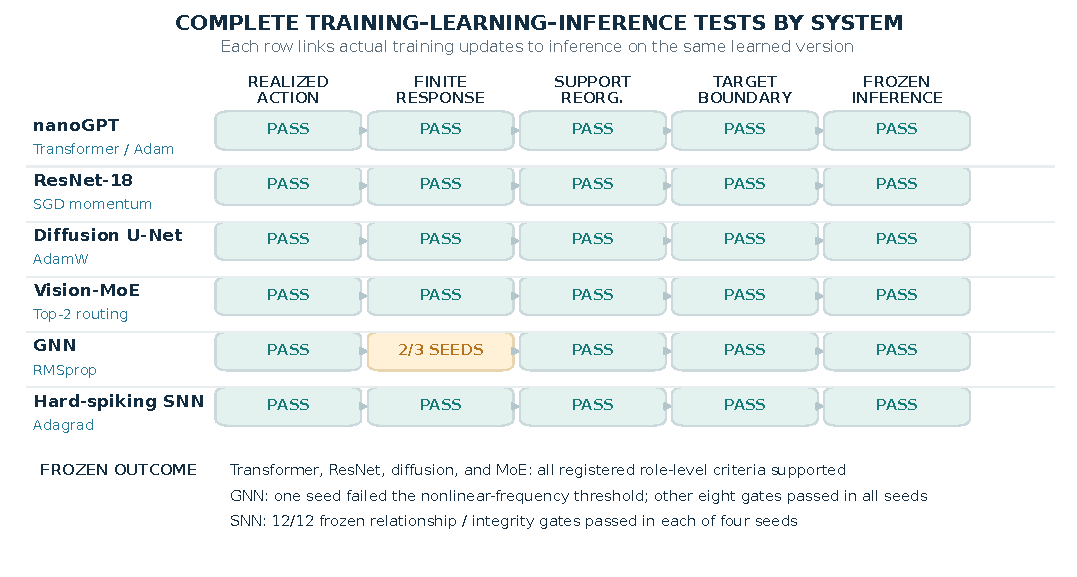
\includegraphics[width=.98\textwidth]{figures/figure2_six_system_evidence.pdf}
  \caption{Within-system training--learning--inference experiment chains. One GNN seed meets eight of nine registered gates, with nonlinear-response incidence below its specified threshold; SNN passes all twelve registered gates in four seeds.}
  \label{fig:systems}
\end{figure*}

\section{Results: Cross-System TLI and Reinforcement}
\subsection{Native Transformer, ResNet, diffusion and MoE chains}
The original nanoGPT program uses realized-update interventions, distributed-support measurements, identity-aligned target transitions, and frozen inference on exact historical trained versions. The frozen inference arm examines thirteen validated histories and 52 selected checkpoints. The post-update target-boundary predictor correctly adjudicates $4{,}652/5{,}088$ confirmation targets (91.43\% accuracy, 91.49\% four-transition macro recall), with errors retained.

On ResNet, all $42/42$ registered parameter receiving-state exchanges exceed the frozen response-difference threshold; 32.23\% of $1{,}536$ target-update response paths meet the nonlinear criterion, and 91.41\% of support records exceed the specified reallocation threshold. Its trained checkpoints then enter the frozen-inference protocol, passed by all three seeds, including learned-version rollback and exact restoration.

On the diffusion U-Net, all $18/18$ parameter-state exchanges exceed the threshold. Nonlinear finite responses occur in 19.25\% of $504$ records, and support reallocation exceeds threshold in 97.02\%. The corresponding frozen-inference protocol passes on all three seeds, including intervention effects in the epsilon predictor and complete 100-step deterministic sampling. This is a generative task with a residual-error capability boundary, rather than another class-label classifier.

The Vision-MoE repeats the connected experiment in a routed-expert organization. All $36/36$ parameter-state and $18/18$ Adam-memory exchanges exceed their registered thresholds; nonlinear paths occur in 35.71\% of $1{,}344$ target-update records, and expert-support reallocation exceeds threshold in 80.43\%. The same final learned versions are tested for deterministic top-2 routing, query-specific expert use, non-additive coalitions, trained expert/router rollback and restoration. The three-seed joint frozen verdict is \texttt{MOE\_UNIFIED\_DYNAMICS\_SUPPORTED}. 

These four systems therefore supply \emph{repeated, within-system} evidence across the action, finite response, support, boundary, and frozen-inference roles. In particular, the inference evidence is linked to training by exact parameter-version identity, not merely by similar behavior in another model.

\subsection{GNN and hard-spiking SNN stress tests}
The GNN experiment performs the same realized-update/receiving-state, finite-path, pre/post coalition-support, target-boundary, and exact learned-version inference sequence. All three formal seeds form the intended capability and pass eight frozen criteria. Two seeds pass the ninth, a $\geq 10\%$ nonlinear-response frequency criterion; one has only $4/256$ qualifying paths (1.56\%) and \emph{fails}. The state-response, support, capability, and frozen-inference measurements were completed across all three seeds.

The hard-spiking SNN uses four recurrent spike components and six temporal steps. Across four formal seeds, all twelve frozen gates pass, including native Adagrad-memory intervention, finite paths, component-support reorganization, query-conditioned inference and exact version rollback. Its discontinuous hard-threshold forward is particularly informative: the connected functional roles remain observable even where a local derivative-based predictor has difficulty modeling threshold crossings. 

\subsection{Reinforcement: feedback-directed support and capability change}
RL-E05/E06 examine the fourth, equally central TLIR role using a shared four-skill GRU policy. All four skills are mastered \emph{before} the matched feedback branches begin; all positive rewards follow the exact two-action task rule. Thus the intervention changes the \emph{distribution of correct feedback}, not reward validity. RL-E05 establishes selective-feedback support concentration, cross-skill interference, and version-sensitive trade-offs, although its stronger registered large-event timing gate was not met.

In RL-E06, 12 formal seeds exhibit strictly dose-ordered changes: from balanced to mild, high, and exclusive feedback, the reinforced skill's mean relative support shares are 25.54\%, 26.47\%, 27.50\%, and 35.20\%, while the other skills' mean margins decrease from 9.474 to 9.130, 8.493, and 3.962. With mild or high concentration, the other skills still achieve 100\% accuracy even though their margins have already eroded. Compared with balanced feedback, exclusive correct feedback shifts support share by +9.67 percentage points and decreases other-skill accuracy by 39.06 points. Rebalancing from the \emph{same} exclusive-update-800 state restores other-skill accuracy from 70.31\% to 99.48\%, while the reinforced skill remains at 100\%. The experiments therefore connect feedback allocation to persistent support reorganization, continuous boundary erosion, observable capability loss, and reversible recovery.

\subsection{Boundary prediction probes both strength and limits}
Direct endpoint prediction measures the accuracy of mathematical approximations alongside the causal intervention tests. Table~\ref{tab:prediction} compares recorded experiments. The primary nanoGPT \texttt{quadratic\_complete} method is adapted to the output and activation structure of each subsequent system.

\begin{table}[t]
\centering
\setlength{\tabcolsep}{4.2pt}
\renewcommand{\arraystretch}{1.13}
\begin{tabular}{@{}lrr@{}}
\toprule
System & Accuracy (\%) & Four-way recall (\%)\\
\midrule
nanoGPT & 91.43 & 91.49\\
ResNet-18 & 99.28 & 97.99\\
Diffusion U-Net & 99.60 & 97.98\\
Vision-MoE & 99.63 & 96.95\\
GNN$^{a}$ & 98.54 & 98.62\\
Hard-spiking SNN$^{a}$ & 95.31 & 70.74\\
\bottomrule
\multicolumn{3}{@{}p{.94\columnwidth}@{}}{\footnotesize $^{a}$Independent prediction tests use registered GNN/SNN training histories.}\\
\end{tabular}
\caption{Post-update target-boundary classification reports. Macro recall averages four observed transition categories; high accuracy alone is not sufficient. Predictor details and evaluation sets differ by system.}
\label{tab:prediction}
\end{table}

For the MoE's direct second-order endpoint predictor, each of the two capability-changing categories contains only nine cases; their high recalls must be interpreted with this limited denominator. On the SNN, the unchanging-boundary baseline already reaches 93.63\% accuracy, and the local formula reaches 95.31\% overall, but only 70.74\% four-way macro recall. Its hard threshold makes true local hidden-state derivatives uninformative about some finite threshold crossings. The lower macro recall isolates a prediction challenge at hard activation thresholds, even as the experimental functional chain remains observable.

\section{Discussion}
TLIR is the complete theoretical account, with Training, Learning, Inference, and Reinforcement as four peer roles. Its TLI relations recur within six architecturally different systems, where exact training histories link realized updates, state-dependent responses, persistent support reorganization, capability readouts, and learned-version frozen inference. The seventh system, a shared GRU policy, probes how Reinforcement changes the future of \emph{already formed} capabilities. This combination tests both the formation/use of support and the feedback that subsequently reorganizes it.

The GRU results reveal why reinforcement can be effective and damaging through the \emph{same functional mechanism}: repeated correct feedback preferentially reallocates support toward the rewarded capability, while unreinforced targets lose continuous readout margin and may later cross into failure. Rebalancing feedback from the same learned state largely reverses this process. Reward correctness alone therefore does not determine whether all previously acquired capabilities are preserved. The evidence concerns controllable support reorganization, not a conserved quantity of support.

Quantitative response patterns remain system-specific: nonlinear-response incidence varies, one GNN seed misses its registered frequency gate, and hard-spiking thresholds challenge local derivative-based prediction. The causal TLI tests and the GRU feedback interventions examine complementary parts of TLIR dynamics; their individual empirical scope should not be confused with requiring every system to reproduce every intervention. Component-level measurements also connect to causal-abstraction analyses of mechanisms \cite{geiger2025}.

\section{Unified Explanations of Positive and Negative Findings}
\label{sec:unified}
\noindent\textbf{Question and discovery order.}
A separate comparison of 21 historical positive/negative pairs asks whether common receiver--action--response--support--boundary--feedback relations explain both the success of local accounts and the findings that limit their scope. The examples below illustrate this shared interpretation.

\noindent\textbf{Kernel dynamics versus feature learning.}
In the corresponding infinite-width lazy regime, NTK dynamics give a rigorous local training description \cite{jacot2018}; feature-learning parameterizations admit different limiting behavior \cite{yang2021}. TLI locates both within receiver- and parameterization-dependent action--response regimes: a valid frozen-kernel projection does not imply that all finite-amplitude training trajectories preserve their features. The two results occupy distinct training regimes.

\noindent\textbf{Sharp minima versus useful sharpness-aware training.}
Function-preserving reparameterizations can change raw parameter sharpness without changing generalization \cite{dinh2017}. Nevertheless, SAM improves performance in specified tasks by optimizing a neighborhood-robust loss \cite{foret2021}. The paired explanation is that raw parameter geometry is not the complete learned functional state, while a sharpness-aware intervention can still change the \emph{actual training action} beneficially. Thus a non-invariant explanatory scalar and an effective local control method can coexist.

\noindent\textbf{Compression as a useful mechanism, not a universal requirement.}
General compression-stage claims fail in some architectures and measurement regimes \cite{saxe2018}, whereas appropriately controlling information bottlenecks can yield valid generalization guarantees \cite{kawaguchi2023}. Persistent functional reorganization in TLI does not require a monotonic decrease of $I(X;T)$, but compression can be one regime-specific outcome of the receiving state, noise, and objective. This predicts \emph{bounded utility without universal necessity}.

\noindent\textbf{Delayed emergence and continued learning after mastery.}
In grokking, test capability can appear abruptly after training performance has saturated, although internal computational structure evolves in identifiable stages \cite{nanda2023}. Neural-collapse results likewise document continuing feature geometry after training error vanishes \cite{papyan2020}. TLI separates persistent support formation from the discrete target readout boundary. Continued internal formation and sudden observable transitions are thus compatible outcomes of the same measured distinction.

\noindent\textbf{Forgetting versus preservation and recovery.}
Continual learning can damage older capabilities, while methods such as EWC protect selected high-importance parameter directions \cite{kirkpatrick2017}. In TLI, the signed response of an old target depends on overlap between the new action and its function-sensitive support, relative to remaining boundary slack. The GRU feedback forks supply a matched intervention example: concentrated \emph{correct} feedback erodes other mastered skills, whereas rebalanced feedback largely restores them. 

\noindent\textbf{Beneficial self-training versus recursive collapse.}
Pseudo-label-based self-training improves accuracy in suitable data mixtures \cite{xie2020}; recursively replacing original data with model-generated samples can instead erase minority tails \cite{shumailov2024}, while accumulating real data can prevent that degradation in studied regimes \cite{gerstgrasser2024}. Both follow a feedback-data distinction: an inference-generated sample is neither intrinsically beneficial nor intrinsically harmful; its retained information and subsequent training action matter. For an under-retained mode with retention factor $0<\rho<1$, a conditional illustrative recursion is
\begin{equation}
 q_{t+1}=(1-\alpha)\rho q_t+\alpha q_{\rm real}.
 \label{eq:feedback}
\end{equation}
At $\alpha=0$ the mode contracts, whereas $\alpha>0$ supplies a positive fixed-point floor if $q_{\rm real}>0$. The recursion models the case of a repeatedly under-retained data mode.

\noindent\textbf{Theory-first extrapolation.}
Beyond historical comparisons, the TLIR relations have been used to derive conditional predictions and their test conditions before searching the relevant literature. Examples include post-capability max-margin selection under exponential-tail losses \cite{soudry2018} and evolving-state stability at the Edge of Stability \cite{cohen2021}. These comparisons identify specific state, action, and boundary conditions under which local mathematical results arise. Future tests can directly intervene on these conditions and evaluate the predicted transitions.

\section{Conclusion}
We investigate the unified Training--Learning--Inference--Reinforcement (TLIR) dynamics of neural systems. Six different architectures repeatedly exhibit the connected TLI relation among realized actions, receiving-state responses, persistent support reorganization, capability boundaries, and exact-version frozen inference. In a seventh, GRU-based system, RL-E05/E06 show that \emph{correct} feedback can selectively concentrate functional support, weaken other mastered capabilities, and reverse these changes when feedback is redistributed. The predictive boundary algorithm and the unified explanations of previously separate positive and negative findings follow from this experimentally grounded TLIR account.

\section*{LLM Usage Statement}
OpenAI ChatGPT was used for research ideation and discussion, assistance with experimental-protocol design and code development/review, interpretation of experimental records, and manuscript drafting, editing, and LaTeX formatting. The authors are responsible for the study design, all scientific claims, and the reported results.


{\small
\bibliographystyle{ieeenat_fullname}
\bibliography{main}
}
\end{document}
